\documentclass[border=6pt]{standalone}
\usepackage{amsmath}
\usepackage{tikz}
\usetikzlibrary{arrows.meta}
\begin{document}
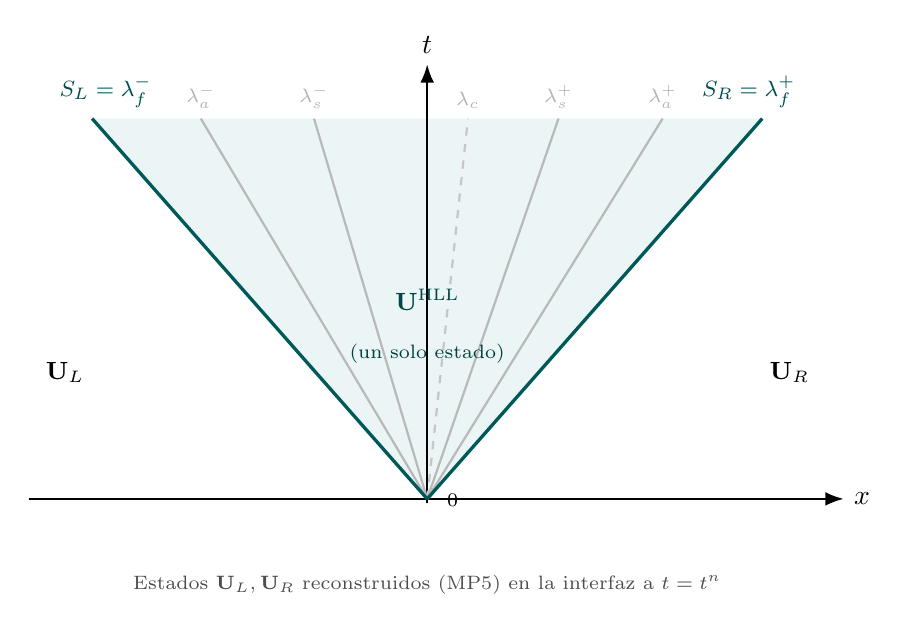
\begin{tikzpicture}[>=Latex,scale=1.15]
\def\T{4.2}
% --- region intermedia HLL (entre S_L y S_R) ---
\fill[teal!8] (0,0) -- (-3.7,\T) -- (3.7,\T) -- cycle;
% --- ejes x-t ---
\draw[->,thick] (-4.4,0) -- (4.6,0) node[right]{$x$};
\draw[->,thick] (0,-0.05) -- (0,\T+0.6) node[above]{$t$};
\node[font=\scriptsize] at (0.28,-0.02) {$0$};
% --- abanico completo RMHD (7 ondas, tenues) ---
\draw[gray!55,thick] (0,0) -- (-2.5,\T) node[above,font=\scriptsize,gray!60]{$\lambda_a^-$};
\draw[gray!55,thick] (0,0) -- (-1.25,\T) node[above,font=\scriptsize,gray!60]{$\lambda_s^-$};
\draw[gray!45,thick,dashed] (0,0) -- (0.45,\T) node[above,font=\scriptsize,gray!60]{$\lambda_c$};
\draw[gray!55,thick] (0,0) -- (1.45,\T) node[above,font=\scriptsize,gray!60]{$\lambda_s^+$};
\draw[gray!55,thick] (0,0) -- (2.6,\T) node[above,font=\scriptsize,gray!60]{$\lambda_a^+$};
% --- ondas rapidas = cotas HLL (gruesas) ---
\draw[very thick,teal!70!black] (0,0) -- (-3.7,\T);
\draw[very thick,teal!70!black] (0,0) -- (3.7,\T);
\node[teal!60!black,font=\footnotesize] at (-3.55,\T+0.3) {$S_L=\lambda_f^-$};
\node[teal!60!black,font=\footnotesize] at (3.55,\T+0.3) {$S_R=\lambda_f^+$};
% --- estados ---
\node[font=\small] at (-4.0,1.4) {$\mathbf U_L$};
\node[font=\small] at (4.0,1.4) {$\mathbf U_R$};
\node[teal!55!black,font=\small] at (0,2.2) {$\mathbf U^{\mathrm{HLL}}$};
\node[teal!50!black,font=\scriptsize] at (0,1.6) {(un solo estado)};
% --- pie ---
\node[align=center,font=\scriptsize,black!70] at (0,-0.95)
  {Estados $\mathbf U_L,\mathbf U_R$ reconstruidos (MP5) en la interfaz a $t=t^{n}$};
\end{tikzpicture}
\end{document}
